\documentclass{beamer}

\usepackage[utf8]{inputenc} % Ensure proper encoding
\usepackage{graphicx} % For including images
\usepackage{hyperref} % For hyperlinks
\usepackage{amsmath,amsfonts,amssymb} % For mathematical symbols and equations
\begin{document}

\title{Workfare versus Welfare: Incentive Arguments for Work Requirements in PovertyAlleviation Programs}
\author{Timothy Besley \& Stephen Coate}
\date{\today}

\frame{\titlepage}


\begin{frame}
\frametitle{Introduction}
\begin{itemize}
\item How should govt design poverty alleviation programs? 
\item Should these programs require a work condition or not?
\item Work requirements provide incentives to earn. Two potential incentives arguments are :
\begin{itemize}
    \item A screening argument that work requirements may serve as a means of targeting transfer.
    \item A deterrent argument that they may serve as a device to encourage poverty-reducing investments
\end{itemize}
\end{itemize}
\end{frame}

\begin{frame}
\frametitle{Screening Argument }
\begin{itemize}
    \item It is very costly to set up a proxy means testing type rule to target poor. It is particularly costly for developing countries that lack the administrative capacity and data.
    \item In such situations, it may be better to make the relief system self-targeting by laying down conditions for claiming support such that only the truly needy present themselves.
    \item Even in developing countries, you might observe the earned income but the potential earnings and therefore there remains an argument for screening through workfare. 
  
\end{itemize}
\end{frame}

\begin{frame}{Deterrence Argument}
\begin{itemize}
    \item This relies on the question whether people are poor by choice i.e, they do not want to work or because of bad luck i.e, they could not find work. 
    \item In case of latter, public assistance can distort incentives (such as divorce if single parents get more benefits). 
    \item Therefore public assistance should be made less attractive by creating some deterrence. 
\end{itemize}
\end{frame}

\begin{frame}[allowframebreaks]{Baseline Poverty Alleviation Program (PAP) with perfect information}
\begin{itemize}
    \item We consider a population consisting of n
 individuals, divided into two types according
 to their income-generating ability or wages, $ a \in
 \{a_L, a_H\},$ where $a_L <a_H $ and where H stands
 for high and L stands for low. A fraction $\gamma$
 has ability $a_L$. Each individual has identical quasi-linear preferences defined over income y and work l. Thus, utility is given by y - h(l) where
 h(.) is increasing and strictly convex.
 \item A PAP is pair of benefits and costs $\{b_i , c_i\}$. $b_i$ is benefit for individual of type i and $c_i$ is the cost. 
 \item The to govt is $n \gamma b_L + n(1-\gamma) b_H$
 \item The govt objective is to minimize cost and ensure each individual gets at least z dollars. 
 \item Both types of individuals choose whether to claim benefits.

    \item The private sector labor supply if individual accepts the program is 
\[
l(b,c,a_i) = 
\begin{cases}
    \hat{l}(a_i) & \text{if } c \leq \hat{l}(a_) \\
    0 & otherwise \\
\end{cases}
\]
where $\hat{l}(a_i)$ is the labor supply of individual of type i in the absence of the program.
\item A work requirement smaller than $\hat{l}(a_i)$ will result in equal reduction in private sector labor supply. 
\item There is no income effect and therefore labor supply is independent of $b_i$.
\item Total private sector earnings given this labor supply are 
\[y(c,a_i)= \begin{cases}
    a_i ( \hat{l}(a_i) - c) & \text{if } c \leq \hat{l}(a_i) \\     
    0 & otherwise \\
\end{cases} \]
\item Therefore total utlity v is 
\[v(b,c,a_i) = b+y(c,a_i) - h(l(c,a_i)+c)\]
\item The individual voluntarily accepts the program if and only if $v(b,c,a_i) \geq v(0,0,a_i)$
\item Assume that only one group will be eligible i.,e $y(0,a_H)>z>y(0,a_L)$.
\item In baseline case, assume that $a_H$ and $a_L$ are exogenous and obserable. Then, policy maker minimizes the cost and follows two constraints: 
\begin{itemize}
    \item Voluntary participation constraint: $v(b,c,a_i) \geq v(0,0,a_i)$ for both types of individuals.
    \item Poor $(a_L)$ must escape poverty and end up with z earnings i.,e $y(c_L,a_L)+b_L \geq z$.
     \end{itemize}

    \item The solution is that high-ability indivdiuals should not get any transfer while low ability individuals should get a transfer of $z-y(0,a_L)$. However, they should not be requird to work as that would just reduce their private sector labor supply and increase benefits while public program do not have any benefit to society. 
    \item This is our benchmark PAP with perfect information.


\end{itemize}

\end{frame}

\begin{frame}[allowframebreaks]{Screening Argument}

    \begin{itemize}
        \item Suppose policy maker cannot observe potential or actual earnings of individuals. 
        \item Then, PAP is not implementable.The optimal policy now depends on govt's information set. There are two cases:
        \begin{itemize}
            \item Govt cannot observe both potential and actual earnings.
            \item Govt can observe actual earnings but not potential earnings.
        \end{itemize}
    \end{itemize}
\end{frame}

\begin{frame}[allowframebreaks]{Unobservable private sector earnings }
\begin{itemize}
    \item Now you need incentive capability constraint that $v(b_L,c_L,a_L) \geq v(b_H,c_H,a_L) $ and $v(b_H,c_H,a_H) \geq v(b_L,c_L,a_H)$. Essentially, we want that each individual to choose the program that is best for them.
    \item If you cannot choose the work requirement, then obvious solution to these constraints is $b_L = b_H$. 
    \item However, with work requirement for low type workers, one can introduce the self-selection. 
\end{itemize}




\begin{figure}  
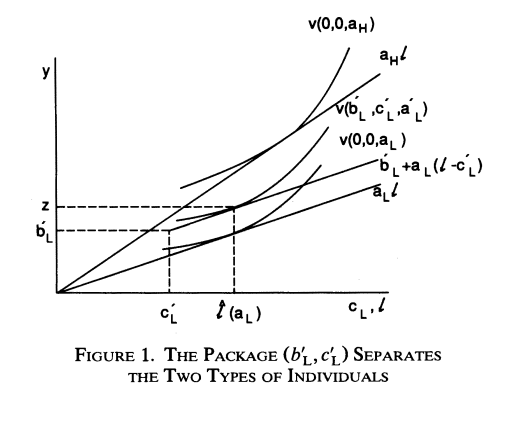
\includegraphics[width=0.8\textwidth]{F1.png}
\end{figure}    

\begin{itemize}
    \item There is now an extra cost because low ability individual reduces private sector labor supply and work c is not productive. So, govt has to balance this trade-off. 
    \item Govt chooses optimal separating work requirement $c^s_L$ such that high ability individuals are indifferent between choosing the program and not choosing the program while at the same time it is sufficient to get the poor to poverty line z. This is given by 
    \[v(0,0,a_H) = v(z-y(c^s_L , a_L), c^s_L,a_H)\]

\item This leads to our 2nd propostion: 

PROPOSITION 2: If both income-generating abilities and incomes are unobservable, one of the following two PAP's is cost minimizing: 
\begin{enumerate}
    \item (welfare) impose no work requirements and offer both ability groups a transfer
 of $z - y(0, a_L)$
 \item  (ii) (workfare) offer self-categorized high-ability individuals no benefits and offer self-categorized low-ability individuals a transfer of $z - y(0, a_L)$ and require them to work $c^s_L$. 
\end{enumerate}
\item The choice between these two solutions trades off the savings from giving no
transfers to the nonpoor against the cost of
reducing the poor's private-sector earnings.
\end{itemize}


\end{frame}

\end{document}
